\section{Fault Modeling}

To determine how different faults manifest themselves in the nominal system with regard to output signals, we first proved a top level property of the nominal WBS using AGREE. This property states: \\

\begin{tt}
If pedals are pressed and no skid occurs, then the brakes will receive pressure. \\
\end{tt}

Using the AADL nominal model and the AGREE contract specification language, this property proves. From this point, we focus our attention on component failures and how this will affect the top level property of the system. 

We would like to specify different component failure modes. These failure modes can be triggered by some internal error or propagated fault. In order to trigger these faults, additional input was added to the AADL model for each fault that can occur within a nominal model component. Our simple fault model contains two types of faults:

\begin{itemize}
\item \textit{fail\_to} fault: This type of failure accounts for both nondeterministic failures and stuck-at failures. The components that are affected by this fault include meter valves and pumps. This fault can be modeled in such a way as to describe both digital and mechanical errors. Examples of digital errors include a \textit{stuck\_at} failure mode for the Command subsystems in the BSCU component. This causes the Command units to become stuck at a previous value. An example of a mechanical error that is captured by this fault is a valve stuck open (or closed). To model this type of fault, the value \textit{alt\_val} can be set to some maximum pressure value for stuck open or zero for stuck closed. This value will then propagate through the system. The definition in AGREE of this fault is shown in Figure~\ref{fig:fail_to_node}.\\

\begin{figure}[h!]
  \centering
 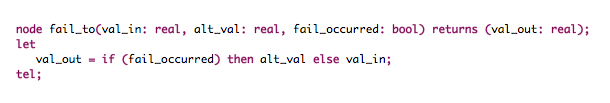
\includegraphics[width=1\textwidth]{images/fail_to.png}
  \vspace{-0.1in}
  \caption{AGREE Definition of a \textit{fail\_to} Fault}
  \label{fig:fail_to_node}
\end{figure}

%%%%%%% DANIELLE
%                     CHECK INTO MECHANICAL FAILURES

\item \textit{inverted\_fail} fault: This type of fault will be used on components which contain boolean output. It will simply take boolean input, negate it, and output the negated value. An examples of this is the Selector. In the nominal model, input to the Selector consists of a boolean value \textit{select\_alternate} value from the BSCU. This value determines the switch of the system from Normal pressure to Alternate pressure. If this value is inverted, the pressure will not be selected according to the requirement description.  See Figure~\ref{fig:inverted_fail_node}

\end{itemize}

\begin{figure}[h!]
  \centering
 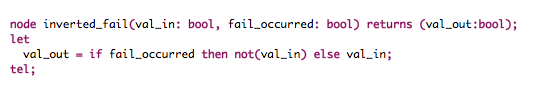
\includegraphics[width=1\textwidth]{images/inverted_fail.png}
  \vspace{-0.1in}
  \caption{AGREE Definition of a \textit{inverted\_fail} Fault}
  \label{fig:inverted_fail_node}
\end{figure}

While modeling these errors, the duration of the fault must also be taken into account. There are both permanent faults and transient faults. We defined an AGREE node called 
\begin{tt}
historically
\end{tt}
which will model the permanent faults based on whether transient faults are historically true. 

The following is a short summary of the failures defined in the fault model. 

\subsection{AADL Faults}
\begin{itemize}

\item Valves and Pumps: All valves and pumps have the possibility of a \textit{fail\_to} fault. This includes Green pump, Blue pump, Accumulator, and the Shutoff valves. 

\item  The Selector can also have a digital \textit{fail\_to} fault regarding the inputs from BSCU commanding to use Normal or Alternate means of pressure along with an \textit{inverted\_fail} fault which would change the boolean value that commands antiskid to activate. 

\end{itemize}

Given our understanding of the AADL system, the assumption was that permanent faults could be introduced into the system and we would still be able to prove our top level property. Upon connecting the faults into the WBS, it was shown that this top level property could not be proven using these permanent faults. Upon further reflection, it was clear why that was the case. 

In the AADL model, the Selector is situated between the pumps and the Blue\_Skid and Green\_Skid components. It's function is as follows: inputs are pump pressures (for Blue, Green, and Accumulator) and information from the BSCU regarding Normal or Alternate pressure. It selects between the Blue and the Green pump in this way. The output of the Selector is pressure of the Blue and Green pumps to the Blue\_Skid and Green\_Skid components respectively. The Blue\_Skid and Green\_Skid components also get a flag from BSCU. Blue\_Skid receives a flag with cmd\_alt while Green\_Skid gets the command cmd\_nor. This will cause those components to either output pressure (if their respective BSCU command is true) or output zero pressure (if the BSCU command is false). The pressure output from here goes directly to the wheel. For a clear picture of this organization, see Figure~\ref{fig:wbs_ima}.

Here is a case when the fault is \textit{fail\_to} and it is a failure of the Green\_Skid component. Previously in the system, the Selector received a command from BSCU to output Normal pressure (Green pump). This command was passed on to the Green\_Skid component along with positive green pressure. If the Green\_Skid component gets stuck at a value of zero for pressure, the output to the wheel is zero. The Blue\_Skid component gets no pressure from the Selector (it has already selected green pressure) and thus outputs no pressure to the wheel. 

Despite one transient failure, the tail end of the system is not designed to recover from this failure. A similar single point of failure is the Blue\_Skid component and the Selector. These faults cause system failure for the same reason. 

\subsection{Strengthening the Nominal Model}
\danielle{Making a figure to put in here showing the additional component of the system.}
To solve this issue, we added a component based on the Simulink model in \cite{Joshi05:Dasc}. This component, the Accumulator\_Valve, takes in the Blue pressure from the Selector and the Accumulator pressure. It also takes in a \textit{select\_alternate} flag from the BSCU. The output of the Accumulator\_Valve goes directly to the Blue\_Skid component and is either the blue or the accumulator pressure. 

An additional piece we added was output to the BSCU from the wheel. The pressure at the wheel is sent to the BSCU to readjust system mode if needed. For instance, if the pressure at the wheel is zero from both blue and green skid components, then the BSCU has a chance to send a \textit{select\_alternate} command over to the Accumulator\_Valve and turn on the accumulator pressure. We assume at this point that we will only use accumulator pressure and not switch back over to Normal mode. 

In order for this to solve the problem, the original top level contract needed to be revisited: 

\begin{tt}
If pedals are pressed and no skid occurs, then the brakes will receive pressure. 
\end{tt}

As it is stated, the added components will not solve the problem. There must be stateful information encoded into this contract. Thus it is changed to: 

\begin{tt}
If pedals are pressed in the previous state and pressed in the current state and no skid occurs, then the brakes will receive pressure. 
\end{tt}

It was also necessary to guarantee that \textit{select\_alternate} is false until an error occurs in the system. This was written as an AGREE guarantee stating that the initialization of \textit{select\_alternate} is false. It remains false until the system commands brake pressure (i.e. brake pedals are pressed), there is no skid occurring, and there is no realized pressure at the wheel. At this point, the system will enter Alternate mode and command pressure from the blue (or accumulator) pump. It will not return to Normal mode. 

















